\chapter{Probleme}

\section{Cuplaj cu costuri pe noduri}

\noindent \textbf{Enunt.} Se da un graf bipartit $G(U + V, E)$ si o functie de cost $w \colon U \to \mathbb{R}$. Sa se determine cuplajul
maximal care maximizeaza suma costurilor nodurilor alese in cuplaj.

\noindent \textbf{Solutie.} Este corect sa prioritizam nodurile in ordinea descrescatoare a costurilor asociate.

\pagebreak

\section{Cuplaj cu costuri pe muchii}

\noindent \textbf{Enunt.} Se da un graf bipartit $G(U + V, E)$ si o functie de cost $w \colon E \to \mathbb{R}$. Sa se determine cuplajul
\textbf{perfect} care maximizeaza suma costurilor muchiilor alese in cuplaj.

\noindent \textbf{Solutie.} Consideram urmatoarea formulare a problemei ca una de programare liniara:

\begin{equation*}
\begin{array}{ll@{}ll}
  \text{max}  & \sum_{(x, y) \in E} w((x, y))m_{x, y} &\\
  \text{s.t.} & \sum_{y} m_{x, y} = 1 \ \forall x &\\
              & \sum_{x} m_{x, y} = 1 \ \forall y &\\
              & m_{x,y} \in \{0, 1\} \ \forall x, y
\end{array}
\end{equation*}

\pagebreak

\section{Izomorfism de subarbori}
\begin{tabular}{l@{\extracolsep{1cm}}l}
  Concurs: & Lot Râmnicu Vâlcea 2015 - Baraj 2 Seniori\\
  Limita de timp: & 0.3\ s\\
  Limita de memorie: & 64\ MB\\
\end{tabular}

\hspace{1cm}

\noindent \textbf{Enunt.} Se dau doi arbori cu radacina in nodul $0$ si cel mult $500$ de noduri, $A$ si $B$.
O operatia consta in stergerea unei frunze. Care este numarul minim de operatii aplicate pe $A$ astfel incat
sa devina izomorf cu $B$?

\noindent \textbf{Solutie.} Cei doi arbori sunt izomorfi daca exista o re-etichetare a nodurilor in asa fel incat sa fie identici.
Consideram mai intai o problema mai simpla: cum vedem daca doi arbori sunt izomorfi? Vom atribui fiecarui arbore un polinom in mai
multe variabile si vom reduce problema la una de echivalenta de polinoame.

\begin{figure}[H]
  \centering
  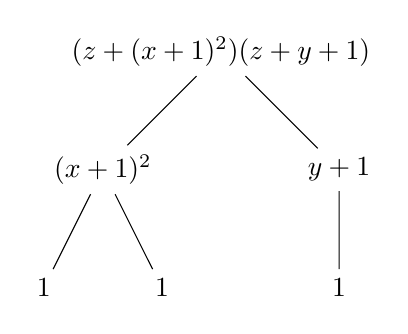
\begin{tikzpicture}[level distance=1.5cm,
    level 1/.style={sibling distance=3cm},
    level 2/.style={sibling distance=1.5cm}]
    \node {$(z + (x + 1)^{2})(z + y + 1)$}
      child {node {$(x + 1)^{2}$}
        child {node {$1$}}
        child {node {$1$}}
      }
      child {node {$y + 1$}
      child {node {$1$}}
      };
  \end{tikzpicture}
  \caption{Constructia polinomului}
\end{figure}

\begin{algorithm}[H]
  \DontPrintSemicolon
  \SetKwFunction{FMain}{DFS-POLY}
  \SetKwProg{Fn}{Function}{:}{}
  \Fn{\FMain{$T$, $u$, $p$}}{
    poly := 1\;
    \For{$v \in T_{u}$}{
      \If{$v \neq p$}{
        poly := poly * ($x_{u}$ + DFS-POLY(T, v, u))\;
      }
    }
    \KwRet poly\;
  }
  \;
\end{algorithm}

Pentru doi arbori, daca evaluam polinoamele cu valori uniform aleatoare alese din $\mathbb{F}_{p}$, atunci probabilitatea de coliziune este de
cel mult $\frac{N}{p}$, unde $N$ este numarul de noduri, conform lemei \textbf{Schwartz-Zippel}. Doi arbori ne-izomorfi vor avea polinoamele diferite
pentru ca inelul polinoamelor $\mathbb{F}_{p}[x_{1}, x_{2}, \ldots, x_{N}]$ determina o factorizare unica a polinomului, descompus intr-un produs de
polinoamele ireductibile si constante.

Avand acest algoritm, putem construi o solutie cu backtracking in care pornind din frunze, eliminam o multime de noduri, mai exact atatea
noduri cat are $A$ in plus fata de $B$ si apoi verificam izomorfismul cu algoritmul dat.

In continuare, observam din solutia precedenta ca raspunsul este fix $|A| - |B|$, daca exista o secventa de operatii. Vom nota cu $a_{v_{1}}$
subarborele nodului $v_{1}$ din $A$ si cu $b_{v_{2}}$ subarborele nodului $v_{2}$ din $B$. Vom construi urmatoarea recurenta folosind
programare dinamica: $d_{v_{1}, v_{2}}$ este adevarat daca putem executa o secventa de operatii astfel incat sa transformam subarborele
nodului $v_{1}$ intr-unul izomorfm subarborelui nodului $v_{2}$ (din celalalt arbore). Este clar ca pentru perechi unde $|a_{v_{1}}| < |b_{v_{2}}|$ valoarea va fi fals. Altfel, consideram fii directi ai acestor doua noduri: $c_{1, 1}, c_{1, 2}, \ldots, c_{1, n_{1}}$ si $c_{2, 1}, c_{2, 2}, \ldots, c_{2, n_{2}}$.
Daca $n_{1} < n_{2}$, atunci nu se poate sa eliminam noduri, micsorand astfel $n_{1}$, incat sa obtinem $n_{2}$. In ce urmeaza ne intereseaza sa gasim o
submultime a fiilor primului nod $c_{1, i_{1}}, c_{1, i_{2}}, \ldots, c_{1, i_{n_{2}}}$ astfel incat $d_{c_{1, i_{j}}, c_{2, j}}$ sa fie adevarate
pentru toti $1 \leq j \leq n_{2}$.

O prima solutie ar fi sa consideram toate cele $\binom{n_{1}}{n_{2}}$ solutii posibile. Aceasta solutie este deja mai eficienta decat prima propusa.

\begin{thm}
  \label{hall}
  \textbf{Hall.} Fie $G = (U \cup V, E)$ un graf bipartit. Exista un cuplaj care acopera $U$ daca si numai daca pentru orice submultime $W$
  a lui $U$, daca consideram multimea $N_{G}(W)$ ca fiind reuniunea vecinilor nodurilor din $W$, atunci $|W| \leq N_{G}(W)$.
\end{thm}

Cum putem folosi \textbf{teorema lui Hall} in cazul nostru este sa construim matricea $d'$ asociata vecinilor lui $v_{1}$, respectiv $v_{2}$
unde $d'_{i, j} = d_{c_{1, i}, c_{2, j}}$. Daca pentru fiecare multime de coloane consideram multimea liniilor care au macar o valoare de adevarat
pe vreuna din coloane, atunci vrem ca numarul de linii sa nu fie mai mic decat numarul de coloane. Aceasta solutie din pacate ramane exponentiala
si se poate construi in timp $O(2^{n_{2}} n_{1})$ daca se proceseaza submultimile de coloane in ordinea codurilor Gray, in timp ce solutia evidenta ar lua
$O(2^{n_{2}} n_{1}n_{2})$. O proprietate inedita a codurilor Gray este ca mastile consecutive de biti vor fi diferite pe fix un bit. Astfel vom determina acel bit,
asociat unei coloane si apoi vom folosi un vector de frecventa pentru a determina ce linii mai raman active pentru noua submultime de coloane, in timp
cel mult $O(n_{1})$.

Problema pe matricea $d'$ este chiar de cuplaj in graf bipartit, iar $d'$ este chiar textbf{matricea Edmonds} (\ref{edmonds}). Ramane sa ii calculam
rangul si sa verificam ca este egal cu $n_{2}$. Complexitatea acestei solutii este:

\begin{equation}
  \sum_{v_{1} \in A} \sum_{v_{2} \in B} n_{1}n_{2}^{2} = \sum_{v_{1} \in A} n_{1} \sum_{v_{2} \in B} n_{2}^{2} \leq |A||B|^{2}
\end{equation}

\noindent pentru ca $a^{2} + b^{2} \leq (a + b)^{2}$.

\pagebreak

\section{Acoperire cu cai a unui graf orientat aciclic}

\noindent \textbf{Enunt.} Se da un graf orientat aciclic $G(V, E)$. Sa se gaseasca o multime de cardinal minim de cai, astfel incat
fiecare nod sa faca parte din exact o cale.

\noindent \textbf{Solutie.} Un graf orientat aciclic este un graf orientat fara cicli orientati. Acesta admite o sortate topologica,
adica o ordonare a nodurilor $v_{1}, v_{2}, \ldots$ in asa fel incat daca exista arcul $(v_{i}, v_{j})$, atunci $v_{i}$ apare inaintea
lui $v_{j}$ in ordonare. Algoritmul pentru a calcula sortarea topologica este urmatorul:

\begin{algorithm}[H]
  \DontPrintSemicolon
  \SetKwFunction{FMain}{DFS-VISIT}
  \SetKwProg{Fn}{Function}{:}{}
  \Fn{\FMain{$G$, $color$, $u$, $T$}}{
    \If{$color_{u}$ = BLACK}{
      \KwRet T\;
    }
    $color_{u}$ := GRAY\;
    \For{$v \in G_{u}$}{
      T := DFS-VISIT($G, color, v, T$)\;
    }
    $color_{u}$ := BLACK\;
    \KwRet [u] + T\;
  }
  \;
\end{algorithm}

\begin{algorithm}[H]
  \DontPrintSemicolon
  \SetKwFunction{FMain}{DFS}
  \SetKwProg{Fn}{Function}{:}{}
  \Fn{\FMain{$G$}}{
    \For{$u \in G$}{
      $color_{u}$ := WHITE\;
    }
    T := []\;
    \For{$u \in G$}{
      T := DFS-VISIT(G, color, u, T)\;
    }
    \KwRet T\;
  }
  \;
\end{algorithm}

\pagebreak

\begin{figure}
  \caption{Contra-exemplu pentru algoritmul de sortare topologica in care se foloseste preordinea.}
  \centering
  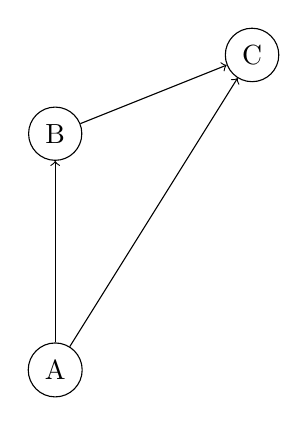
\begin{tikzpicture}
    \node[shape=circle,draw=black] (A) at (0,0) {A};
    \node[shape=circle,draw=black] (B) at (0,3) {B};
    \node[shape=circle,draw=black] (C) at (2.5,4) {C};

    \path [->] (A) edge node[left] {} (B);
    \path [->](B) edge node[left] {} (C);
    \path [->] (A) edge node[left] {} (C);
  \end{tikzpicture}
\end{figure}

Algoritmul practic construieste inversa postordinii si aceasta este chiar o sortare topologica posibila.
Nu este corect sa consideram preordinea, asa cum reiese din exemplul urmatorul unde este posibil sa inseram $C$
inaintea lui $B$ daca este vizitat inainte din $A$.

Avand calculata sortarea topologica, o prima solutie cu backtracking va considera nodurile in ordinea inversa.
Ne putem imagina caile ca o colorare, iar acum la fiecare pas al algoritmului trebuie sa stabilim culoarea pentru
nodul curent. Pentru ca le procesam in ordinea inversa sortarii topologice, stim ca am procesat deja toti vecinii lui
iar acestia sunt colorati in culorile $\{C_{1}, C_{2}, \ldots, C_{k}\}$. Pentru a asigura invariantul de cale, odata ce
un nod preia culoarea unui vecin, vecinul isi pierde culoarea si nu mai poate fi ales pe masura ce coboram in adancime.
Atunci, pentru nodul curent trebuie sa alegem una din aceste culori sau sa cream o culoare noua. Dupa ce toate nodurile
au fost colorate putem sa ne uitam la numarul de culori diferite folosite si aceasta va fi un candidat pentru raspunsul
problemei.

\begin{lem}
  Complexitatea acestei solutii este de $O(|E|2^{|V|})$.
\end{lem}

\begin{proof}
  In cel mai rau caz, consideram nodurile in ordine si la fiecare pas avem o decizie, ne atasam la o cale existenta sau cream o cale
  noua.
\end{proof}

\noindent Solutia polinomiala a problemei nu este evidenta, dar este sugerata de conexiunea cuplajului in graf bipartit cu teorema lui
Dilworth. Vom numi o \textbf{anticale} o secventa de noduri $v_{1}, v_{2}, \ldots, v_{k}$ pentru care
$\forall \ v_{i}, v_{j} \ (v_{i}, v_{j}), (v_{j}, v_{i}) \notin E$.

\begin{thm}
  \label{Dilworth}
  \textbf{Dilworth.} Numarul minim de cai necesare ca sa acoperi graful este egal cu marimea celei mai lungi anticai.
\end{thm}

\begin{thm}
  \label{Konig}
  \textbf{Kőnig (1931).} In orice graf bipartit, numarul de muchii dintr-un cuplaj maximal este egal cu numarul de noduri din acoperirea minima.
\end{thm}

Avand aceasta observatie, este mai clara reducerea la cuplaj in graf bipartit. Construim graful bipartit in care dublam fiecare nod din graful
initial astfel incat sa apara in ambele multimi. Apoi, muchiile din graful initial le vom considera si in acesta, doar ca vor conecta doar
noduri din multimi diferite. Acum, daca am gasi o multime maxima de noduri independente, aceasta va fi o \textbf{anticale}.

\pagebreak

\section{Bilingual}

\begin{tabular}{l@{\extracolsep{1cm}}l}
  Concurs: & Google Code Jam 2015 Round 2\\
  Limita de timp: & 10\ s\\
  Limita de memorie: & 256\ MB\\
\end{tabular}

\hspace{1cm}

\noindent \textbf{Enunt.} Se dau $N + 2 \ (2 \leq N \leq 200)$ liste de cuvinte. Se stie ca prima lista contine doar cuvinte in limba
engleza, a doua contine doar cuvinte in limba franceza. Restul de $N$ nu se cunosc si trebuie catalogate intr-una
din cele doua limbi in asa fel incat sa se minimizeze numarul de cuvinte care fac parte in ambele limbi.

\hspace{1cm}

\noindent \textbf{Solutie.} O prima solutie cu backtracking trebuie sa asocieze fiecarei liste o limba si apoi sa
verifice numarul de cuvinte care se afla in ambele limbi. Sunt $2^{N}$ posibilitati de a alege, iar verificarea poate
dura si pana la suma numarului de cuvinte, daca acestea se normalizeaza in prealabil. Sunt mai multe moduri in care
putem imbunatati constanta acestei solutii. In primul rand, putem ignora cuvintele care nu apar in mai mult de o
propozitie. De asemenea, in cazul acestui backtracking, o alta optimizare semnificativa ar fi iterative deepening pe raspuns,
adica sa nu urmarim ramuri care cresc numarul de cuvinte incompatibile din raspuns imediat ce le observam (depth-first),
dar sa o abordam gradual si sa preferam o crestere in latime, nu in adancime. Din pacate aceasta solutie nu este destul
de rapida, nici macar pentru anul $2015$, cand solutiile la Code Jam se rulau local si se cerea doar rezultatul unei
rulari de program.

Problema se aseamana unei probleme clasice de taietura minima, numita \textbf{Image segmentation}. Taietura minima este duala
problemei de flux maxim. In aceasta problema sunt $N$ pixeli. Fiecarui pixel $i$ se poate asocia o culoare de prim plan de cost
$f_{i}$ sau o culoare de fundal $b_{i}$. Daca doi pixeli $i$ si $j$ sunt adiacenti si au asocieri diferite, atunci trebuie scazuta
o valoare $p_{i,j}$. Problema cere sa se efectueze asocierile in asa fel incat sa maximizeze costul. Fie $P$ multimea pixelilor carora
le-a fost asociat prim-planul si $Q$ multimea pixelilor carora le-a fost asociat fundalul, atunci dorim sa maximizam
$\sum_{i \in P} f_{i} + \sum_{i \in Q} b_{i} - \sum_{i \in P, j \in Q \lor i \in Q, j \in P} p_{i,j}$. Aceasta se poate reformula ca o problema
de minimizare a valorii $\sum_{i \in P, j \in Q \lor i \in Q, j \in P} p_{i,j}$. Reteaua de flux maxim dubleaza nodurile pentru fiecare pixel
in asa fel incat un nodul $2u$ inseamna $u$ a fost asociat pe prim-plan, iar $2u+1$ inseamna $u$ a fost asociat pe fundal. Sursa este
conectata catre toate nodurile de prim-plan $2u$ cu capacitate $f_{u}$, iar destinatia este conectata catre toate nodurile de fundal $2u+1$
cu capacitate $b_{u}$. Muchii de capacitate $p_{i,j}$ se adauga intre nodurile adiacente de asocieri diferite. A taietura de la sursa la
destinatie este apoi o asociere a pixelilor in multimile $P$, respectiv $Q$.

In cazul nostru, culoarea de prim plan inseamna un cuvant in limba engleza, iar culoarea de fundal inseamna un cuvant in limba franceza.
Observam ca nu ne intereseaza valorile $f_{i}, b_{i}$, trebuie doar sa fie suficent de mari, iar valoarea de ``penalty'' se aplica atunci cand
un cuvant este asociat in ambele limbi si are cost $1$. Trebuie totusi sa avem grija sa nu atribuim mai multe limbi aceleiasi liste, asadar mai
asociem un cost $\inf$ intre cuvinte de limba diferita din aceeasi propozitie. Trebuie tratate cu atentie cuvintele din primele doua propozitii.

In schimb, nu am prezentat degeaba aceasta problema. Ea poate fi rezolvata mai departe si ca o problema de cuplaj maxim in graf bipartit.
Putem imparti cuvintele in trei multimi, cuvintele care sunt doar in engleza, cuvintele care sunt doar in franceza si cuvintele
care sunt in ambele limbi. Pentru a minimiza numarul de cuvinte din ambele limbi ne dorim sa maximizam numarul de cuvinte care sunt intr-o
singura limba. Ca inainte, vom construi doua noduri pentru fiecare cuvant $u$, nodul $2u$ va fi ales daca $u$ nu este un cuvant in engleza,
iar nodul $2u + 1$ va fi ales daca $u$ nu este un cuvant in franceza. Pentru fiecare doua cuvinte $u_{1}, u_{2}$ din aceeasi lista adaugam o
muchie intre $2u_{1}$ si $2u_{2} + 1$. Ramane de gasit cea mai mare multime de noduri astfel incat nu exista o muchie intre nicio pereche, adica
\textbf{maximal independent set}. Pe caz general aceasta nu se poate rezolva polinomial, insa graful creat este evident unul bipartit. In grafurile
bipartite \textbf{maximal independent set} este complementul acoperirii minime cu nodurilor (\textbf{minimal vertex cover}).

Asadar, folosind \ref{Konig}, putem folosi algoritmul de cuplaj maximal \ref{Algoritm paralelizabil pentru cuplaj} pentru a calcula raspunsul problemei.

\pagebreak

\section{Paritatea numarului de cuplaje}
\begin{tabular}{l@{\extracolsep{1cm}}l}
  Concurs: & Olimpiada nationala pentru studenti 2015, Runda finala\\
  Limita de timp: & 1\ s\\
  Limita de memorie: & 20\ MB\\
\end{tabular}

\hspace{1cm}

\noindent \textbf{Enunt.} Se da un graf bipartit $G = (U + V, E)$ unde $|U|, |V| \leq 100$. Sa se determine paritatea numarul de cuplaje perfecte.

\hspace{1cm}

\noindent \textbf{Solutie.} Este clar ca daca $|U| \neq |V|$ atunci numarul este $0$, deci par. Altfel, putem pentru inceput sa testam fiecare permutare, in complexitate $O(|U|!)$.

Putem imbunatati solutia precedenta daca o abordam cu programare dinamica. Construim tabela $D_{i, S}$ care este paritatea numarului de cuplaje a
primelor $i$ elemente din $U$ cu multimea de noduri din $S \subseteq V$. Recurenta se poate construi astfel:

\begin{equation}
  D_{i, S} = \sum_{(u_{i}, v_{j}) \in E} D_{i-1, S - \{v_{j}\}} \mod 2
\end{equation}

\noindent Aceasta solutie are complexitate de timp $O(2^{|U|} (|U| + |E|))$

\begin{thm}
  Numarul de cuplaje perfecte este egal cu permanentul matricei Edmonds asociat.
\end{thm}

\begin{proof}
  Permanentul unei matrice patratica $A$ de marime $N \times N$ este egal cu $\sum_{P \in S_{N}} \prod_{i=1}^{N} A_{i, P_{i}}$.
  Valoarea $\prod_{i=1}^{N} A_{i, P_{i}}$ este $1$ daca si numai daca $P$ este un cuplaj perfect. Insumam aceasta valoare
  pentru toate permutarile. Deci am numarat cuplajele perfecte.
\end{proof}

Se observa, din formula, ca permanentul este determinantul ``fara semn''. Totusi, atunci cand lucram in $\mathbb{F}_{2}$,
semnul nu conteaza, pentru ca $-1 \mod 2 = 1$. Asadar, pentru a afla paritatea numarului de cuplaje, este de ajuns sa
determinam paritatea determinatului. Pentru aceasta, putem folosi metoda Eliminarii Gauss in $\mathbb{F}_{2}$, in complexitate
$O(\frac{N^{3}}{w})$, unde $w$ este marimea unui cuvant. Pana acum nu se cunoste vreun algoritm polinomial pentru a calcula
permanentul pe caz general.

\pagebreak

\section{Divisible Matching}

\begin{tabular}{l@{\extracolsep{1cm}}l}
  Concurs: & CS Academy Round \#67\\
  Limita de timp: & 4\ s\\
  Limita de memorie: & 256\ MB\\
\end{tabular}

\hspace{1cm}

\noindent \textbf{Enunt.} Se da un graf bipartit $G(U \cup V, E)$ cu $1 \leq |U| = |V| \leq 100$,
un numar intreg $2 \leq K \leq 100$ si o functie pentru a determina valoarea unei muchii
$f : E \to \{0, 1, \ldots, K-1\}$. Sa se determine daca exista un cuplaj perfect $M$,
astfel incat $K \ | \ \sum_{e \in M} f(e)$.

\hspace{1cm}

\noindent \textbf{Solutie.} Fara a pierde din generalitate, presupunem ca $|U| = |V| = N$.
O solutie evidenta in complexitate $O(N!)$ construieste si verifica toate permutarile din $S_{N}$.
Chiar daca le procesam in ordine aleatoare, numarul asteptat de pasi este tot de ordinul $N!$. \\
Urmatoarea solutie pe care o putem aborda este sa optimizam solutia de backtracking mentionata anterior
cu metoda programarii dinamice. Construim tabela $D_{i,\text{rem}, S}$ ca fiind o valoare booleana daca poti
cupla nodurile $\{u_{1}, u_{2}, \ldots, u_{i}\}$ din $U$ cu nodurile $S \subseteq V$ astfel incat restul sumei
valorilor muchiilor alese de pana acum, modulo $K$ este rem. Recurenta cu care se poate construi este:

\begin{equation}
  D_{i, \text{rem}, S} = \bigvee_{j \in S \wedge e_{i, j} = (u_{i}, v_{j})} D_{i-1, \text{rem} - f(e_{i, j}), S - \{\j\}}
\end{equation}

\noindent Din pacate solutie ramane exponentiala, complexitatea acesteia fiind $O(KN^{2}2^{N})$.

\pagebreak

In ce urmeaza ne putem gandi sa rezolvam o subproblema mai simpla, mai exact cea in care $K=2$.
Ne intereseaza un cuplaj cu numar par de muchii de $1$. Daca privim muchiile cu $1$ ca fiind
rosii, iar celelalte ca fiind albastre, atunci obtinem problema \textbf{cuplajului rosu-albastru} (\ref{redbluematching}),
in care ne intereseaza doar ca numarul de muchii rosii sa fie par. In ce urmeaza ne vom concentra pe varianta
in care folosim lema Schwartz-Zippel. Avand \textbf{matricea Edmonds} $A$ construita special pentru acest caz,
$\det(A)$ este un polinom monic in variabila $y$. Atunci cand voiam sa aflam daca exista un cuplaj cu numar
fix de muchii rosii, interpolam $\det(A)$ si verificam daca $y^{k}$ are un coeficient nenul. In cazul de fata
ne intereseaza daca exista macar un termen $y^{k}$ cu coeficient nenul, iar $k$ par. O prima varianta este sa
interpolam polinomul pentru fiecare numar par, insa putem face mai eficient. O metoda sa aflam suma coeficientilor
pari ai unui polinom $p$ este sa evaluam $\frac{p(1) + p(-1)}{2}$. Desigur, in cazul nostru, acest calcul se
efectueaza tot intr-un corp finit si putem sa obtinem iar $0$ pentru ca s-au anulat coeficientii adunatii.
Din fericire, putem aplica iar lema Schwartz-Zippel sa obtinem ca acest fapt este, in continuare, indeajuns
de improbabil.

Pentru a continua sa rezolvam problema pentru orice $K$, amintim ca insumarea coeficientilor divizibil cu o anumita valoare
se poate face folosind \textbf{filtrarea prin radacini ale unitatii} (\ref{rootsofunityfilter}). Problema este insa
sa gasim un corp potrivit care are radacini ale unitatii de ordinul $K$. Daca nu gasim in timp util, mai putem sa extindem
corpul in asa fel incat sa introducem $\zeta \neq 1$ pentru care $\zeta^{K} = 1$. Insa, daca abordam asa, operatiile
aritmetice vor dura $O(K^{2})$ (sau macar $O(K \log K)$ daca folosim algoritmi de aritmetica "state of the art"),
in loc de $O(1)$, unde tinteam. Corpul pe care il cautam va fi $\mathbb{F}_{p}$, unde $p$ este un numar prim pentru care
$p \mod k = 1$. Pe modelul RAM operatiile aritmetice in $\mathbb{F}_{p}$ dureaza $O(1)$. Presupunem ca generatorul acestui
corp este $g$, pe care il putem gasi cu \textbf{algoritmul pentru radacini primitive} \ref{primitiveroot}. Stim ca
$\phi(p) = p - 1$, deci $g^{p - 1} = 1 \mod p$, iar $k\ |\ p - 1$, deci $\zeta = g^{\frac{p-1}{k}}$.

Complexitatea acestei solutii este acum $O(K W(N))$, unde $W(N)$ este timpul necesar calculului de determinant si este
de ajuns sa se incadreze in limitele date.

\section{Xor Matching}

\begin{tabular}{l@{\extracolsep{1cm}}l}
  Concurs: & Codechef September Challenge 2018 Division 1\\
  Limita de timp: & 2\ s\\
  Limita de memorie: & 2\ GB\\
\end{tabular}

\hspace{1cm}

\noindent \textbf{Enunt.} Se da o matrice $A$ de marime $N \times N \ (1 \leq N \leq 60)$ cu valori intregi in celule
din multimea $\{0, 1, \ldots, 1023\}$. Se considera toate permutarile de coloana ale matricei $A$ si se calculeaza
$A_{1, 1} \oplus A_{2, 2} \oplus \ldots \oplus A_{N, N}$, unde $\oplus$ este operatie de xor pe biti.
Sa se determine ce valori se pot obtine.

\hspace{1cm}

\noindent \textbf{Solutie.} O prima solutie este sa consideram toate cele $N!$ permutari ale coloanelor si sa se calculeze
valorile.

O imbunatatire a solutiei precedente este sa aplicam programare dinamica. Mai exact, vom contrui recurenta $D_{i, \text{sum}, S}$
ca fiind o valoare booleana care indica daca putem permuta pentru primele $i$ linii coloanele din multimea $S$ astfel incat sa
suma xor pana acum sa fie egala cu $\text{sum}$. Recurenta este urmatoarea:

\begin{equation}
  D_{i, \text{sum}, S} = \bigvee_{j \in S} D_{i, \text{sum} \oplus A_{i, j}, S - \{j\}}
\end{equation}

Solutia ramane apoi in acele valori adevarate $\text{sum}$ din $D_{N, \text{sum}, \{1, 2, 3, \ldots, N\}}$. Complexitatea acestei solutii
este $O(N^{2}2^{N}\max(A))$, care din pacate nu este destul de rapida pentru restrictiile date.

La prima vedere nu este evidenta relatia pe care problema o are cu cuplajul in grafuri bipartite. Insa daca privim liniile matricei ca
o secventa de noduri $u_{1}, u_{2}, \ldots, u_{N}$, iar coloanele $v_{1}, v_{2}, \ldots, v_{N}$, atunci $A$ este matricea de adiacenta a
unui graf bipartit in care exista o muchie intre oricare doua noduri $u_{i}, v_{j}, 1 \leq i, j \leq N$ de valoare $A_{i, j}$.

Vom incerca sa rezolvam o problema mai simpla acum, mai exact cazul cand $\max(A) = 1$. In acest caz, putem obtine suma xor $0$ daca exista
un cuplaj cu numar par de muchii de valoare $1$, iar suma $1$ daca exista un cuplaj cu numar impar de muchii de valoare $1$. Aceasta subproblema
aduce aminte la problema cuplajului rosu-albastru (\ref{redbluematching}). Ca pana acum, vom considera varianta cu lema Schwartz-Zippel pentru
simplitatea operatiilor aritmetice. Avand \textbf{matricea Edmonds} $A$ construita special pentru acest caz,
$\det(A)$ este un polinom monic in variabila $y$. Atunci cand voiam sa aflam daca exista un cuplaj cu numar
fix de muchii rosii, interpolam $\det(A)$ si verificam daca $y^{k}$ are un coeficient nenul. In cazul de fata
ne intereseaza daca exista macar un termen $y^{k}$ cu coeficient nenul, iar $k$ e par pentru cazul cu suma
xor $0$, iar impar pentru cazul cu suma xor $1$.
